\documentclass[12pt]{article}

\usepackage{a4wide}
\usepackage[utf8]{inputenc}

\usepackage{graphicx}

\pagestyle{empty}

\parindent=0pt

\begin{document}

\section*{Diskrétní Fourierova transformace}

Na cvičení se pokusíme naprogramovat diskrétní Fourierovu transformaci (DFT).
V dalším cvičení se pak pokusíme o zpětnou transformaci.

Fourierova transformace spočívá ve výpočtu frekvenčního spektra zadaného vstupního obrazu $f$, které označujeme $F$ (jedná se o komplexní matici s rozměry vstupního obrazu).

\begin{equation}
    F(k, l) = \sum\limits_{m=0}^{M-1} \sum\limits_{n=0}^{N-1} f(m, n) \varphi_{k, l}(m, n)\,.
\end{equation}

Báze $\varphi_{k, l}$ je definována následovně

\begin{equation}
    \varphi_{k, l}(m, n) = \frac{1}{\sqrt{MN}} e^{-i 2 \pi \left( \frac{mk}{M} + \frac{nl}{N} \right) }, k = 0, 1, \dots, M-1 \,\, \mathrm{a} \,\, l = 0, 1, \dots, N-1\,.
\end{equation}

Abychom při výpočtu báze nemuseli stále počítat odmocninu, hodnoty vstupního obrazu
normalizujeme touto odmocninou. Bázi pak počítáme bez této normalizace.
Pro výpočet báze je vhodné využít Eulerova vzorce $e^{ix} = \cos( x ) + i \sin( x )$.
Díky tomuto vzorci se nám řešení již v této fázi dělí na reálnou a imaginární část. Přesněji tedy:

\begin{equation}
    F(k, l) = R(k, l) + I(k, l)\, .
\end{equation}

Amplituda spektra $|F(k, l)|$ je 

\begin{equation}
    |F(k, l)| = \sqrt{ R^2(k, l) + I^2(k, l)}\, .
\end{equation}

Fázový posuv spektra $\Phi(k, l)$ je 

\begin{equation}
    \Phi(k, l) = \mathrm{arctg}\left( \frac{I(k, l)}{R(k, l)} \right)\, .
\end{equation}

Energetické spektrum signálu $P(k, l)$ (power spectrum) je možno vypočítat jednoduše jako $|F(k, l)|^2$.

\begin{equation}
    P(k, l) = |F(k, l)|^2\, .
\end{equation}

Energetické spektrum signálu je možno zobrazit tak, že jej logaritmujeme a výsledné hodnoty normalizujeme do rozsahu $\langle 0, 1\rangle$. Abychom dobře viděli energetické spektrum, je dobré prohodit 1. s 3. kvadrantem a 2. s 4. kvadrantem. Toto se nám také bude hodit pro aplikaci filtrů ve frekvenční doméně.
\\
\\
\textbf{Hint:} Pracujete s datovým typem \textbf{\texttt{double}} pro reprezentaci vstupního obrazu, prvků frekvenčního spektra i fázového posuvu.

\section*{Očekávaný výstup}

\begin{center}
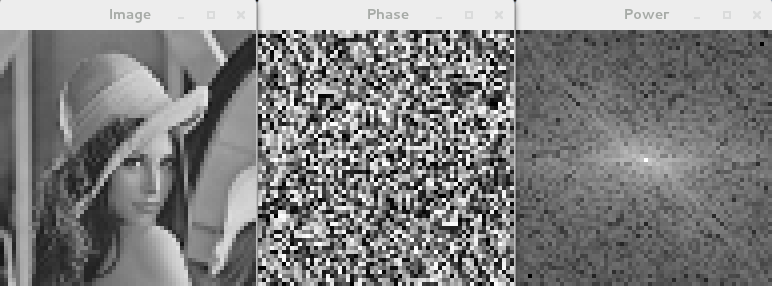
\includegraphics[width=0.8\textwidth]{result_images.png}
\end{center}

\end{document}

